%=========== ΛΥΣΗ - ΘΕΜΑ Β_96 ===========
\begin{thema}{Β}
Στο παρακάτω αναβαθμισμένο σχήμα σημειώνονται οπτικά τα σημεία τομής, η σχετική θέση των δύο καμπυλών, και η σκιασμένη περιοχή του ζητούμενου εμβαδού μεταξύ τους.
\begin{center}
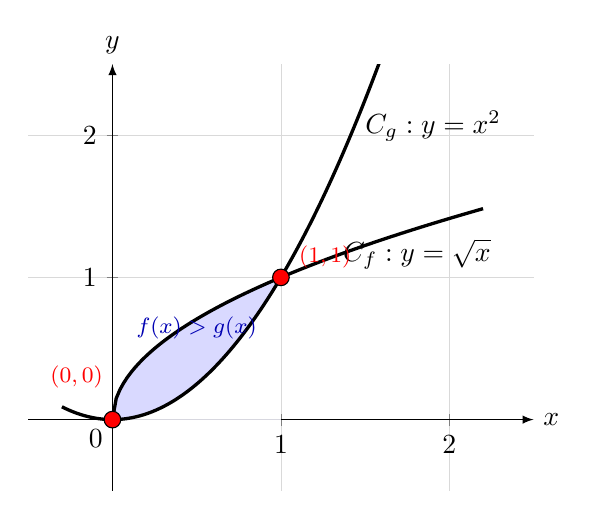
\begin{tikzpicture}
    \begin{axis}[axis lines = middle,
        axis line style = {->, >=latex},
        grid = major,
        grid style = {very thin, gray!30},
        xlabel = {$x$},
        ylabel = {$y$},
        xtick = {1,2,3},
        ytick = {1,2,3},
        every axis x label/.style = {at={(current axis.right of origin)}, anchor=west},
        every axis y label/.style = {at={(current axis.above origin)}, anchor=south},
        width = 8cm, height = 7cm, samples = 100,
        xmin=-0.5, xmax=2.5, ymin=-0.5, ymax=2.5,
        xtick distance=1, ytick distance=1
    ]
        % Σκιασμένο Χωρίο (f πάνω, g κάτω)
        \addplot[fill=blue!15, draw=none, domain=0:1] {sqrt(x)} \closedcycle;
        \addplot[fill=white, draw=none, domain=0:1] {x^2} \closedcycle;
        
        % Καμπύλες
        \addplot[very thick, \xrwma, domain=0:2.2] {sqrt(x)} node[pos=0.85,below] {$C_f: y=\sqrt{x}$};
        \addplot[very thick, black, domain=-0.3:1.6] {x^2} node[pos=0.85,right]{$C_g: y=x^2$};
        
        % Σημεία τομής
        \addplot[mark=*, mark options={fill=red, scale=1.5}] coordinates {(0,0)};
        \addplot[mark=*, mark options={fill=red, scale=1.5}] coordinates {(1,1)};
        \node[anchor=south east, color=red, font=\footnotesize\bfseries] at (axis cs:0, 0.15) {$(0,0)$};
        \node[anchor=south west, color=red, font=\footnotesize\bfseries] at (axis cs:1.05, 1) {$(1,1)$};
        
        % Σχολιασμός ανισότητας
        \node[anchor=south, color=blue!70!black, font=\footnotesize\bfseries] at (axis cs:0.5, 0.5) {$f(x) > g(x)$};
        
        \node[below left] at (axis cs:0,0) {$0$};
    \end{axis}
\end{tikzpicture}
\end{center}

\begin{erwthma}

\item Τα σημεία τομής αναγνωρίζονται οπτικά στις θέσεις όπου οι δύο καμπύλες αλληλοτέμνονται. Από τον κάναβο, τα σημεία τομής βρίσκονται στο $(0, 0)$ και στο $(1, 1)$. Οι αντίστοιχες τετμημένες τομής είναι $x = 0$ και $x = 1$.

Για τη γραφική λύση της ανίσωσης $f(x) > g(x)$, αναζητούμε πού η γραφική παράσταση $C_f$ βρίσκεται \textbf{πάνω} από την $C_g$. Παρατηρώντας, αυτό συμβαίνει στο ανοιχτό διάστημα $(0, 1)$, δηλαδή μεταξύ των δύο σημείων τομής. Άρα, $f(x) > g(x) \Leftrightarrow x \in (0, 1)$.

\item Το εμβαδόν του χωρίου μεταξύ δύο συνεχών καμπυλών στο διάστημα από $x = 0$ ως $x = 1$ εκφράζεται ακριβώς ως:
\[ E = \int_0^1 |f(x) - g(x)| \,\mathrm{d}x \]
Εφόσον δείξαμε ότι στο $(0, 1)$ η $f$ βρίσκεται πάνω, ισχύει $f(x) - g(x) \ge 0$, άρα η απόλυτη τιμή αφαιρείται και παίρνουμε:
\[ E = \int_0^1 \bigl( f(x) - g(x) \bigr) \,\mathrm{d}x \]

\item Αντικαθιστούμε τους αναλυτικούς τύπους $f(x) = \sqrt{x}$ και $g(x) = x^2$:
\[ E = \int_0^1 \left( \sqrt{x} - x^2 \right) \mathrm{d}x = \int_0^1 x^{1/2} \,\mathrm{d}x - \int_0^1 x^2 \,\mathrm{d}x \]
\[ = \left[ \frac{x^{3/2}}{3/2} \right]_0^1 - \left[ \frac{x^3}{3} \right]_0^1 = \left[ \frac{2}{3} x^{3/2} \right]_0^1 - \left[ \frac{x^3}{3} \right]_0^1 \]
\[ = \frac{2}{3} \cdot 1 - \frac{1}{3} = \frac{2}{3} - \frac{1}{3} = \frac{1}{3} \ \text{τ.μ.} \]

\item Η μέγιστη κατακόρυφη απόσταση στο $(0, 1)$ αντιστοιχεί στη μέγιστη τιμή της $h(x) = f(x) - g(x) = \sqrt{x} - x^2$ στο $(0, 1)$.
Παραγωγίζοντας:
\[ h'(x) = \frac{1}{2\sqrt{x}} - 2x \]
Θέτοντας $h'(x) = 0$:
\[ \frac{1}{2\sqrt{x}} = 2x \Leftrightarrow 1 = 4x\sqrt{x} \Leftrightarrow 1 = 4x^{3/2} \Leftrightarrow x^{3/2} = \frac{1}{4} \Leftrightarrow x = \left(\frac{1}{4}\right)^{2/3} = \frac{1}{4^{2/3}} = \frac{1}{2^{4/3}} \]
Η θέση αυτή ανήκει στο $(0, 1)$. Υπολογίζουμε τη μέγιστη τιμή:
\[ h\!\left(\frac{1}{2^{4/3}}\right) = \frac{1}{2^{2/3}} - \frac{1}{2^{8/3}} = \frac{1}{2^{2/3}} - \frac{1}{2^{8/3}} = \frac{2^2 - 1}{2^{8/3}} = \frac{3}{2^{8/3}} = \frac{3}{4\sqrt[3]{4}} \approx \frac{3}{6{,}35} \approx 0{,}47 \]
Δεδομένου ότι $\frac{3}{4\sqrt[3]{4}} < \frac{3}{4 \cdot 1} = \frac{3}{4}$, χρειαζόμαστε ένα πιο λεπτομερές φράγμα.
Ισχύει $\sqrt[3]{4} > 1{,}587$, οπότε $4\sqrt[3]{4} > 6{,}35$, που δίνει $\dfrac{3}{4\sqrt[3]{4}} < \dfrac{3}{6} = \dfrac{1}{2}$. 
Συνεπώς, $h(x) < \dfrac{1}{2}$ για κάθε $x \in (0, 1)$, πράγμα που σημαίνει ότι η μέγιστη κατακόρυφη απόσταση μεταξύ $C_f$ και $C_g$ στο $(0, 1)$ είναι πράγματι \textbf{μικρότερη από $\frac{1}{2}$}.

\end{erwthma}
\end{thema}
%=========== ΤΕΛΟΣ ΛΥΣΗΣ - ΘΕΜΑ Β_96 ===========
